
\documentclass[letterpaper, 10 pt]{ieeeconf}  
% Comment this line out if you need a4paper
%\documentclass[a4paper, 10pt, conference]{ieeeconf}      
% Use this line for a4 paper

\IEEEoverridecommandlockouts                              
% This command is only
% needed if you want to
% use the \thanks command

\overrideIEEEmargins

\usepackage{graphicx} 
\usepackage[utf8x]{inputenc}
\usepackage[spanish]{babel}
\usepackage{fancyhdr}
\usepackage{epic}
\usepackage{eepic}
\usepackage{amsmath,amsfonts}
\usepackage{threeparttable}
\usepackage{amscd}
\usepackage{here}
%\usepackage{subfigure}
\usepackage{lscape}
\usepackage{tabularx}
\usepackage{longtable}
\usepackage{color}
\usepackage{tikz}
\usepackage{hyperref}
\usepackage{rotating}


\title{\LARGE \bf
A Stochastic High-Resolution Dynamic Model for the Assessment of Realtime Forest Fire Susceptibility.}

\author{E. Zapata$^{1}$, N Velasquez$^{2}$, C.D. Hoyos, S. Ospina}% <-this % stops a space


\begin{document}

\maketitle
\thispagestyle{empty}
\pagestyle{empty}


%%%%%%%%%%%%%%%%%%%%%%%%%%%%%%%%%%%%%%%%%%%%%%%%%%%%%%%%%%%%%%%%%%%%%%%%%%%%%%%%
\begin{abstract}

\end{abstract}

%%%%%%%%%%%%%%%%%%%%%%%%%%%%%%%%%%%%%%%%%%%%%%%%%%%%%%%%%%%%%%%%%%%%%%%%%%%%%%%%
\section{INTRODUCTION}
Forest fires at the Aburra Valley watershed (VA) have caused several forest losses (CITAS), health issues for the residents (CITAS) and increases in the $CO_2$ emissions \citep{Andreae2001}. At the VA, human activities along with weather oscillations affect the occurrence of forest fires, and the efforts to reduce them have shown limited success due to access and public order issues (hay CITAS?). The mentioned characteristics limit event attention and increase the need for prevention strategies.  This prevention goes from educational strategies (CITAS) to technological implementations such as cameras, human monitoring, and models (CITES).\\

With the use of models, it is possible to produce predictions that eventually help the prevention strategies CITAS.  However, according to several studies (CITAS) forest fires vulnerability is explained by the vegetation and its moisture, the weather, the hydrology, and human activities. Each one of the described factors includes its variability and uncertainties that decreases its predictability from a physical point of view CITAS. Due to this, several authors have tried to develop empirical forest fires prediction models (CITAS). HABLAR DE LAGUNOS DE LOS MODELOS QUE HAY.\\

Along with the models, there are efforts in order to observe, monitor, and measure forest fires.  At a global scale, \citep{Fearnside2018} used Landsat and OLI satellite images to monitor forest fires on the Amazonas basin for 33 years. In a more local case, \citep{Valero2017} use unmanned vehicles to track on live fires and eventually improve forest fires accuracy. There are also efforts to analyze detailed information about forest fires at pine forest \citep{ElHoussami2017}, grasslands \citet{Roger2015}, shrublands \citet{Santoni2006}, and forested environments \citet{Wotton2012}. Besides, there is also fire live monitoring by using cameras \citep{Bao2015}. Some of these monitoring efforts involve multiple methodologies CITAS and are usually used along with models for decision making CITAS.\\

In the VA region, forest fires are likely to happen during the dry season of December, January, and February. Due to the land cover and topographical characteristics, forest fires last between several hours to 2 days.  Moreover, their covered area is limited to 30 $ha$.  Considering these characteristics, we develop a strategy that involves monitoring, modeling, and warning. The monitoring consists of 12 forest fires detection cameras along with three high-resolution thermal cameras distributed along the valley.  Also, we develop a Bayesian dynamic model that predicts forest fire vulnerability distributed and at an hourly scale. For the setup of the model, we use static and dynamic information.   Through the cameras and the model, a continuous monitoring strategy is established, which is transmitted to the authorities in real time.

PARRAFO CON LA ESTRUCTURA DEL ARTICULO.




\section{Study region and data}
 
\subsection{Study area}

The forest fire strategy was deployed in the VA watershed located in Colombia in the department of Antioquia (see Figure \ref{fig:ubicacion}). With an area of 1040$km^2$ with and urban development of the 40$\%$ and a population of 7M, VA houses the City of Medellin (the capital city of Antioquia) and other nine municipalities. Fires usually happen at the grasslands, small crops, and tropical vegetation located around the urban area (see critical regions Figure \ref{fig:ubicacion}).\\

\begin{figure}[h]
\centering
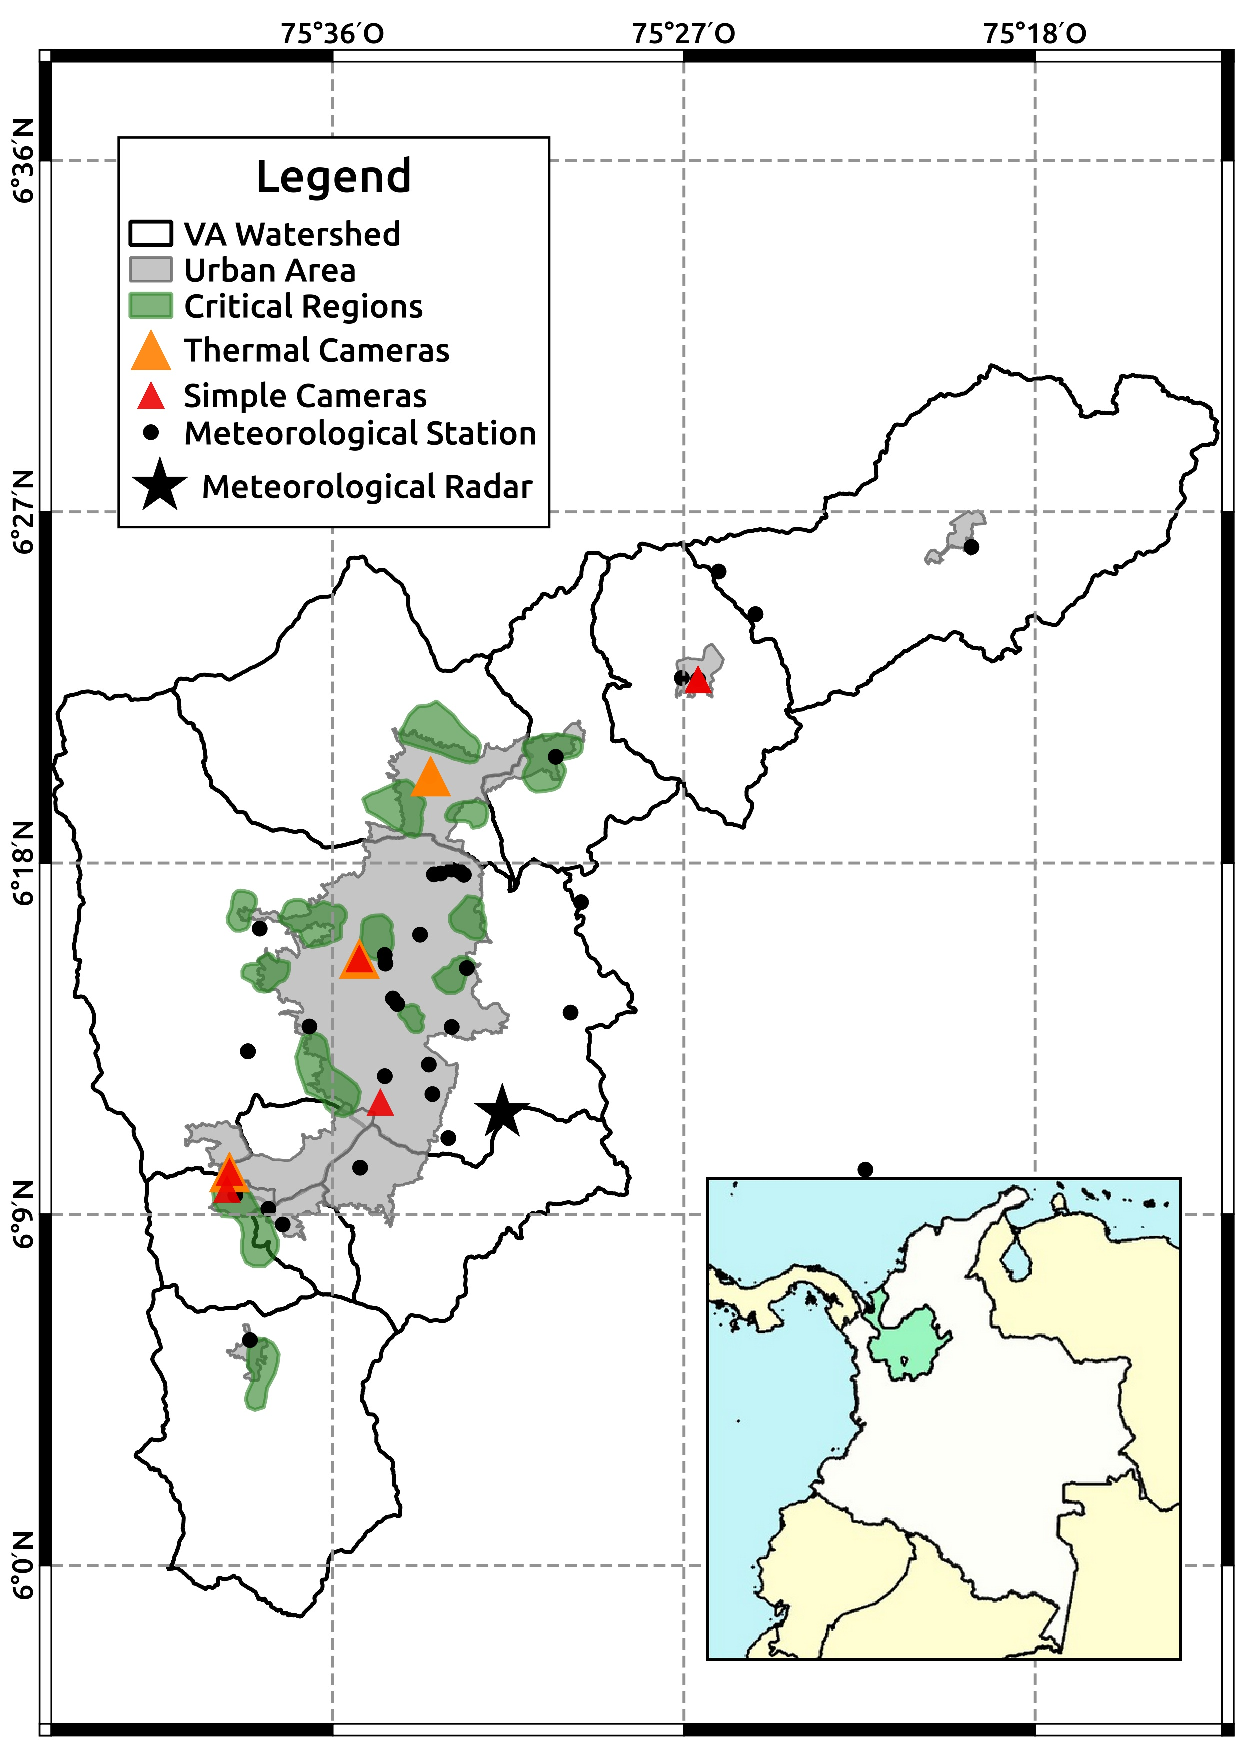
\includegraphics[trim={0.2cm 0cm 0.2cm 0cm},clip,width=8.0cm]{Figuras/map_intro_cameras.pdf}
\caption{Location Aburra Valley, critical zones for historical occurrences, high resolution cameras for monitoring and meteorological data.}
\label{fig:ubicacion}
\end{figure}

\subsection{Data}

For the fires modeling and monitoring, we use static and dynamic data.  In order to monitor 24/7, we use heat and high-definition cameras (Figure \ref{fig:ubicacion}). On the other hand, the model relies on static and dynamic raster maps data. We consider that static variables exhibit almost no change over time and are updated occasionally.  On the other hand, the dynamic variables change at each time step.\\     

The static variables consider a human interaction layer, a layer considering land use, and a layer of historical critic regions of forest fires occurrence (see Figure \ref{fig:staticLayers}). The human interaction (Figure \ref{fig:staticLayers}a) considers the vegetation fire susceptibility regardless of the climatic conditions.  These activities include urban expansion, crops expansion, roads construction, and tourism.  On the other hand, the land use layer (Figure \ref{fig:staticLayers}b) was obtained through a supervised classification of the Pleiades sensor (CITA). In this layer, we consider vegetation, grass, forest, crops, bare soil, and water bodies. Finally, the historical critic layer considers the historical occurrence of the forest fires in the last ten years.\\

\begin{figure*}
  \centering
  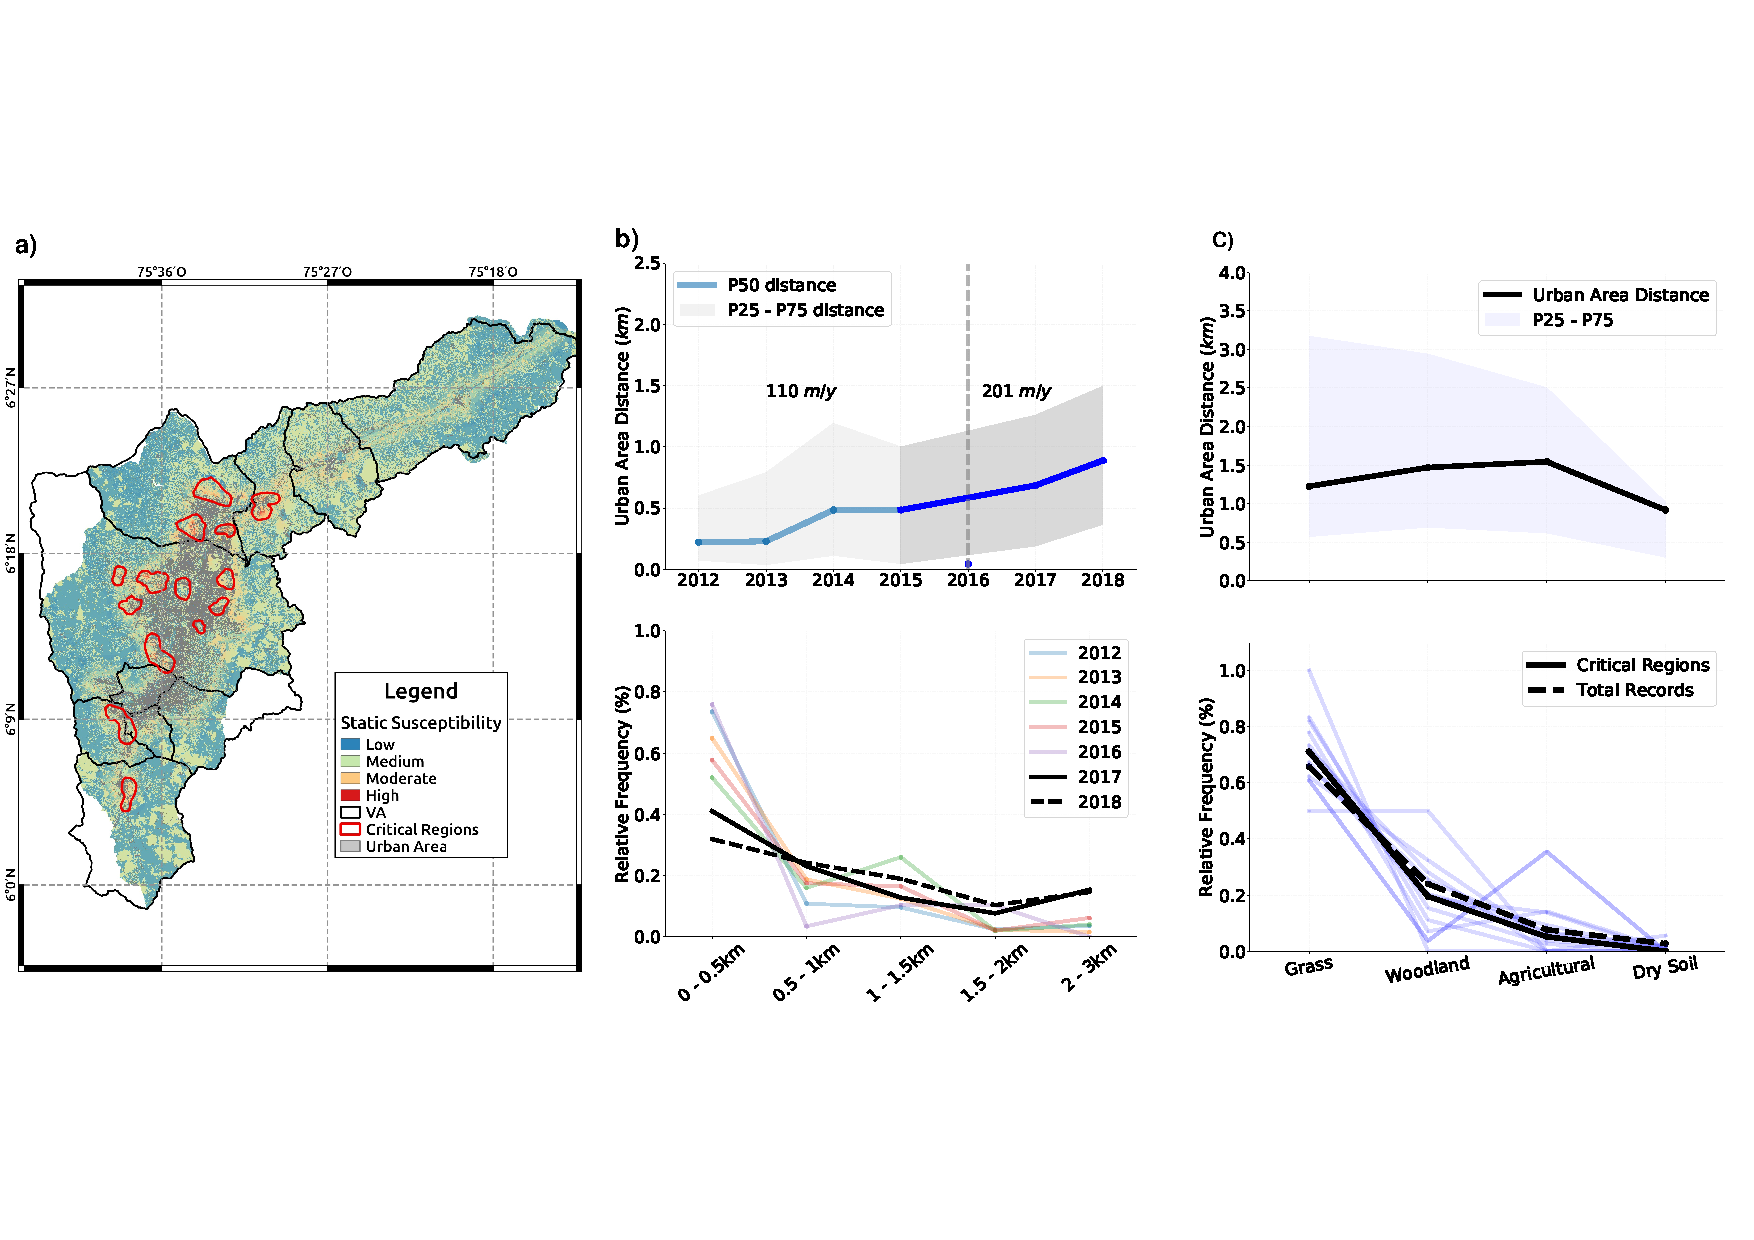
\includegraphics[width=1.0\linewidth]{Figuras/static_composition1.pdf}
  \caption{Static layer. Human interaction, land use and historic occurrence.}
  \label{fig:staticLayers}
\end{figure*}

The dynamic variables change over time, and they depend on climatic conditions. These variables include soil moisture, a product derived from rainfall, and an estimation of the superficial temperature. The soil moisture (Figure \ref{fig:dynamicLayers}a) is the result of an open loop hydrology model CITA. The rainfall product (Figure \ref{fig:dynamicLayers}b) is the result of the cumulative rainfall of the last ten days weighted by the elapsed time between its occurrence and the present. With this two variables, the model has an estimation of the moisture contained on the vegetation crucial to determine the vegetation forest fire vulnerability CITA. Additionally, we include a superficial temperature estimation (Figure \ref{fig:dynamicLayers}c).  The temperature is obtain from the WRF model CITA at two meters of the surface at a spatial resolution of 2$km$.\\

\begin{figure*}
  \centering
  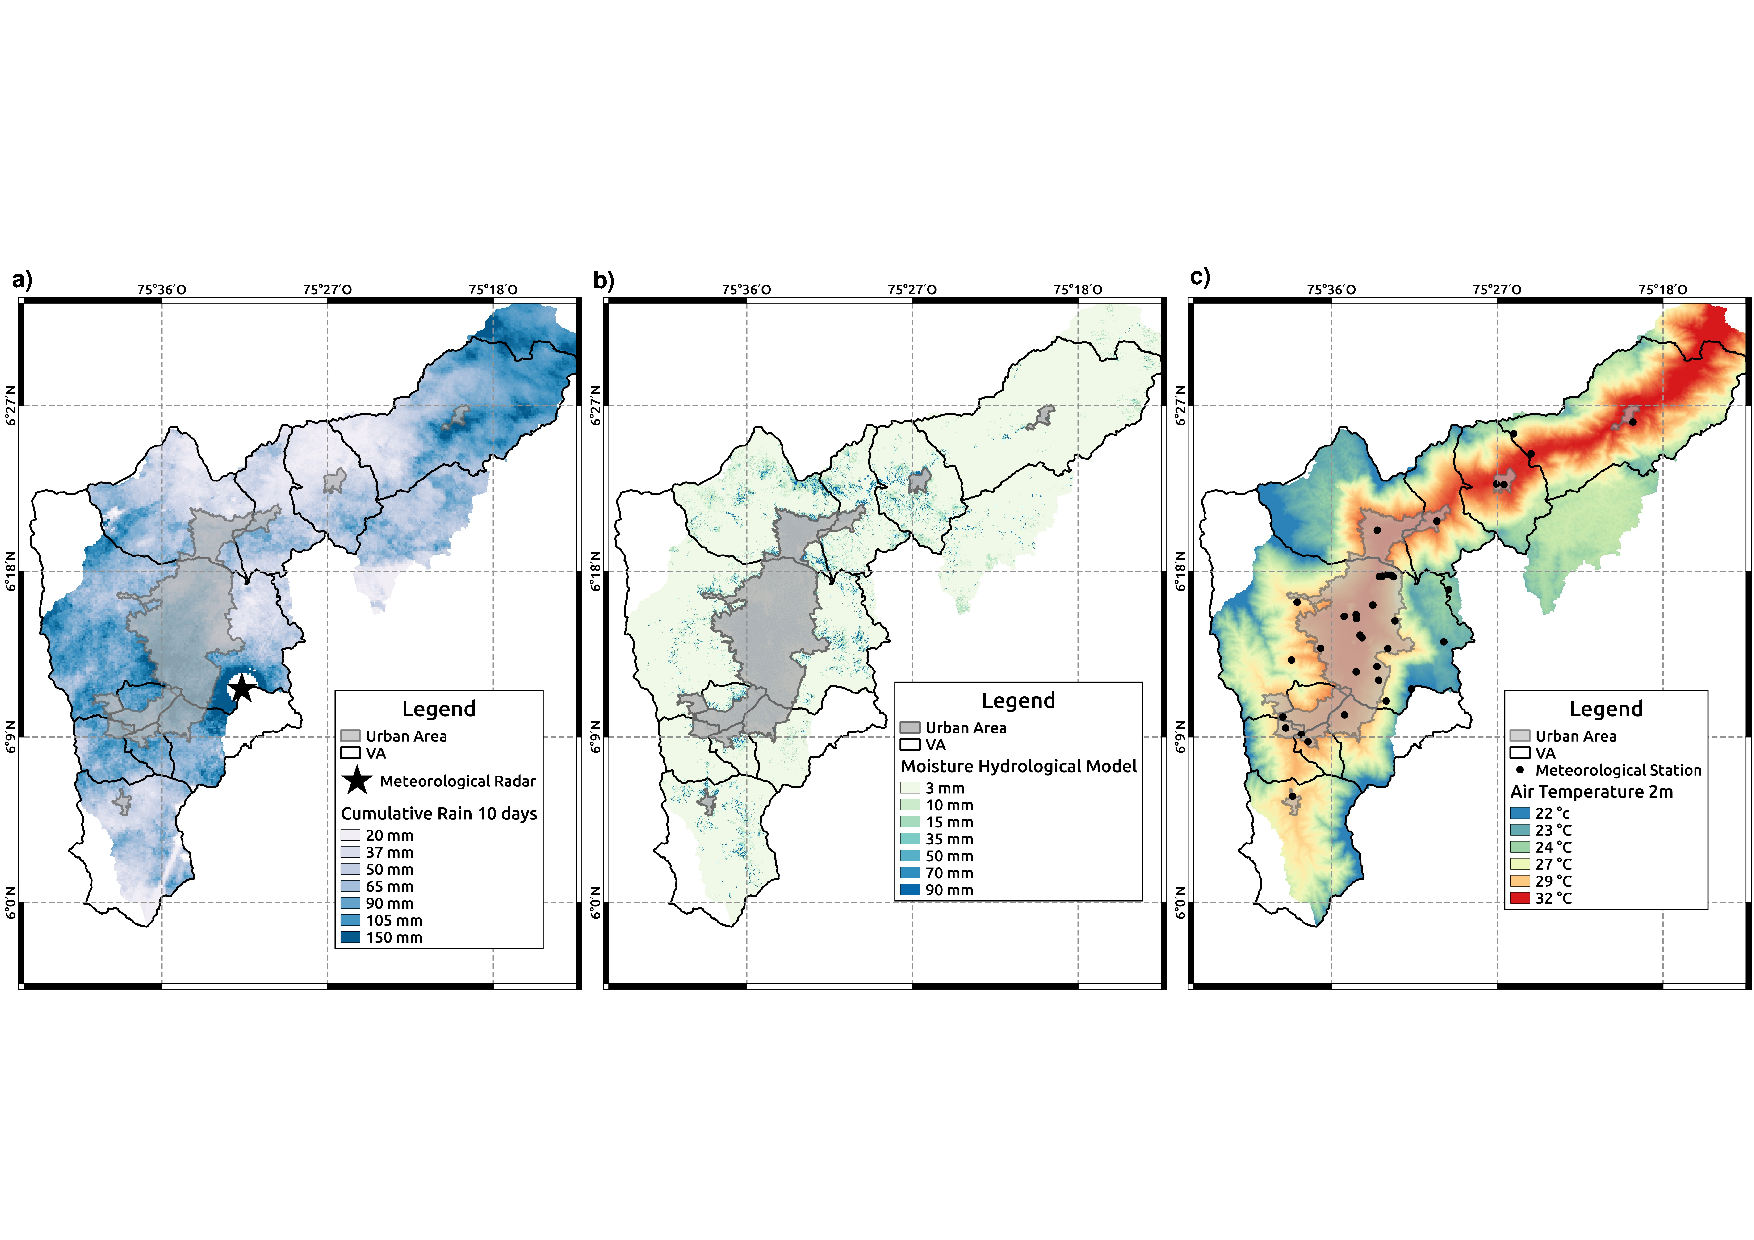
\includegraphics[width=1.0\linewidth]{Figuras/dynamic_composition1.pdf}
  \caption{Dynamic layer. Cumulative rain 10 days, soil moisture and surface temperature.}
  \label{fig:dynamicLayers}
\end{figure*}

In the Table \ref{Tab:info_all} we show a summary of the information used for the development of the strategy and the model. Both, temporal and spatial resolution change from variable to variable (column 3 at Table \ref{Tab:info_all}), however, when used, the temporal scale is fixed to 1 hour and the spatial scale to 60m. 

\begin{table}[!h]
\label{Tab:info_all}
\caption{Information}
\begin{tabular}{| c | c | c | c | c |}
\hline
\textbf{Parameter} & \textbf{Type} & \textbf{Scale} & \textbf{Resolution} & \textbf{Source} \\
\hline

Surface Temperature  (2m) & WRF Model & 2 km & Hourly & SIATA \\ \hline
Air Temperature  & Recorded & Punctual Value  & 1 Minute & SIATA \\ \hline
Rain 10 days & Radar  & 150 m & 5 minutes & SIATA \\ \hline
Soil Moisture & Map & 60m & 5 minutes & SIATA \\ \hline
Land Use & Map & 50 cm & Fixed & SIATA \\ \hline
Wildfire Records & Database &  Events & Fixed & Fire Brigades\\
Recorded wildfires & Database & Events & SIATA \\
\hline

\end{tabular}
\end{table}

\section{Methodologies}

\section*{Forest fires susceptibility model}

For the model we use the variables described at the data section. For the model, each variable is aggregated to a spatial resolution of $60m$ and converted to an occurrence probability map. Then, the vulnerability index map $SI(t)$ is obtained as a weighted sum of the variables: 

 \begin{equation}
     SI = MS \cdot W_{1} + MP \cdot W_{2} +MH \cdot W_{3}
     \label{eq:weighted}
 \end{equation}

From equation (\ref{eq:weighted}), $MS$ is a map that summarizes the static variables derived from three maps: human interaction $HI$ , land use $LU$ , and critic zones $CZ$. The $HI$ map was obtained by analyzing historic forest fires at increasing buffers from the urban area (FIGURA?). The $LU$ map, stands for the occurrence probability in function of the vegetation type. And $CZ$ was estimated in function of the last 10 years records. $MS$ is equal to the sum of the described maps (equation (\ref{eq:estatico}) each one mapped to a range of 0 to 1. $MS$ is also used as a decision taker product, for which it is categorized into low, mid-low, mid-high, and high susceptibility.\\

The human interaction map $HI$ was derived from historic records between 2012 and 2016, and it has representative dynamics that must be considered.  According to the records, critical regions tend to be localized around the urban perimeter (red polygons at Figure \ref{fig:distance_urban}a). The distance between fires and the urban area has increased through the years, however, the higher probability is still below 1000 m (see  Figure \ref{fig:distance_urban}b).  The described trend is possible explained by the increase of both: the urban area and the monitoring. However, to assess the effect of the urban expansion we perform an analysis using historic NDVI data from 1996 to 2018.\\    

In this analysis, we classify each NVDI map as a binary map with 1 as urban development and 0 as vegetation.  Then, we sum the classified maps obtaining an approximation to the evolution of the urban development in the recent years. Figure \ref{fig:porc_ndvi} shows the obtained map in the analysis, values near 22 correspond to an urban development with high rate, and values equal to 0 correspond to no urban development. Also, at Figure \ref{fig:evol_ndvi} we present, the temporal evolution of the urban development, which shows an increase of the 30\% over the last years.     




The model also considers temporal dynamic variables.  The rainfall variable $MP$ uses accumulated radar-rainfall fields for the last 10 days. From historic records, $MP$ is the occurrence probability given a total rainfall amount in the last ten days. The soil moisture map $MH$ is derived from the operational hydrological model of SIATA. This map, considers the soil moisture variability due to sub-surface flow and evaporation. Finally we use a land surface temperature variable map $MT$ as a mask, based on this map, the model only considers suceptibility for values above XX $^oC$.\\

In addition to the maps, the model uses a set of weights $W_i$ to determine the susceptibility. The values of $W_i$ must be adjust to obtain a high accuracy with the lowest possible number of false positives. Here we explain our procedure to obtain the values of $W_i$.\\
 
 \begin{itemize}
     \item[1] We start with NNN number of observed historic forest fires.  Each fire has a date and a localization.  
     
     \item[2] For each date $d$ we obtain the dynamic maps $MP(d)$ and $MH(d)$.  The static map is fixed for this process.  
     
     \item[3] We produce a uniform random generation of 1000 groups of weights $G(W_1, W_2, W_3)$. With the considered events, each group $G$ has a number of successes $Ns$ and a number of false positives $Nf$.
     
     \item[4] Finally, we select a group that has a high value of $Ns$ with the lowest possible value of $Nf$.
 \end{itemize}



\section*{MONITORING}

EL MONITOREO CON CAMARAS DE ALTA RESOLUCIÓN UBICADAS EN SITIOS ESTRATEGICOS DE LA CIUDAD PERMITE LA IDENTIFICACIÓN 24/7 DE LOS INCENDIOS EN COBERTURA VEGETAL, LOS CUALES SON REPORTADOS A LOS ORGANISMOS DE RESPUESTA Y TOMADORES DE DECISIONE. EL MONITOREO ES COMPLEMENTADO CON SOBREVUELOS CON DRONE PARA APOYAR EN LAS ACTIVIDADES DE EXTINCIÓN Y OBTENER DE PRIMERA MANO PARTICULARIDADES DEL EVENTO; ZONA AFECTADA, VEGETACIÓN INVOLUCRADA, ESTABLECER POSIBLES RAZONES, ETC.\\

LOS REGISTROS SON ALMACENADOS PARA REALIZAR VALIDACION CONSTANTE DEL MODELO DE SUSCEPTIBILIDAD. ADICIONALMENTE SE GENERAN REPORTES DIARIOS, SEMANALES Y MENSUALES QUE AGRUPAN MODELACIÓN, MONITOREO Y RESPUESTA.\\

PARA EL MONITOREO DE LAS LADERAS SE DISPONE DE NN CAMARAS DE ALTA RESOLUCION, NN CAMARAS TERMICAS (REFERENCIA) Y NN VISIBLES (REFERENCIA). EN LA FIGURA XX SE PRESENTA LA COBERTURA OBTENIDA CON EL TOTAL DE CAMARAS. EN LA TABLA XX SE PRESENTAN LAS CARACTERISTICAS TECNICAS DE CADA UNA DE LAS CAMARAS.\\

\textbf{FIGURA COBERTURAS}\\
\textbf{TABLA CAMARAS}

\section*{ALERTS}

EL MODELO DE SUSCEPTIBILIDAD QUE SE PRESENTA EN ESTE TRABAJO ES PUBLICADO ES GENERADO CON FRECUENCIA HORARIA Y ES COMPARTIDO TRES VECES AL DIA CON LOS ORGANISMOS DE SOCORRO. ESTO EN CONJUNTO CON EL MONITOREO 24/7 DE LAS LADERAS DEL VA POR MEDIO DE LA RED DE CAMARAS PERMITE GENERAR ALERTAS TEMPRANAS PARA LA PREVENCION Y ATENCION DE INCENDIOS EN COBERTURA VEGETAL. ADICIONALMENTE EN LA ATENCION DE EVENTOS SE REALIZAN SOBREVUELOS PARA OBTENER INFORMACION DE DIRECCION Y VELOCIDAD DE PROPAGACION, CARACTERIZACION DE AREA AFECTADA, RUTAS DE ACCESO, ETC.\\

HASTA ACA DATOS!!!!!!!!!!!!


\begin{figure}[h]
\centering
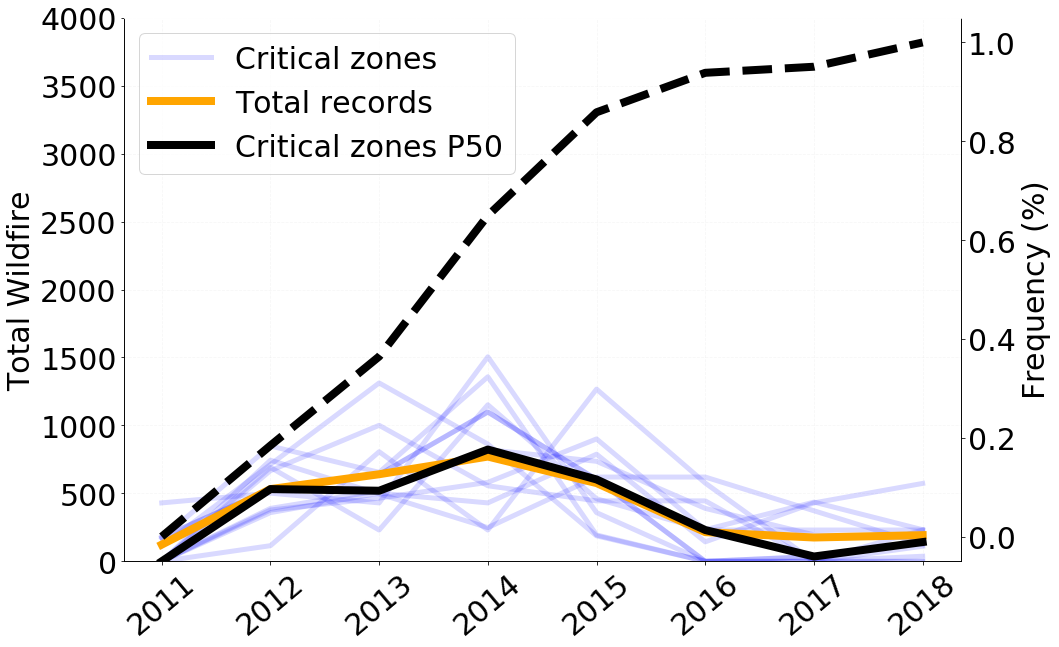
\includegraphics[width=9.0cm]{Figuras/historical_wildfire.png}
\caption{Evolution of the number of forest fire events reported at the VA in the last N years.}
\label{fig:incendiosAno}
\end{figure}

En el planteamiento del modelo las variables utilizadas se dividen en dinamicas y estaticas en función de su variabilidad en el tiempo.

En este trabajo se utilizan campos de radar para estimar acumulados de lluvia y para  modelación hidrológica de la humedad del suelo, además de una red de estaciones meteorólogicas en el Valle de Aburrá. El radar meteorológico y la red meteorológica son operadas por el Sistema de Alerta Temprana de Medellín y el Valle de Aburrá (SIATA).



\subsection{Static Data}

\subsection*{Interacción antrópica}




\begin{figure}[h]
\centering
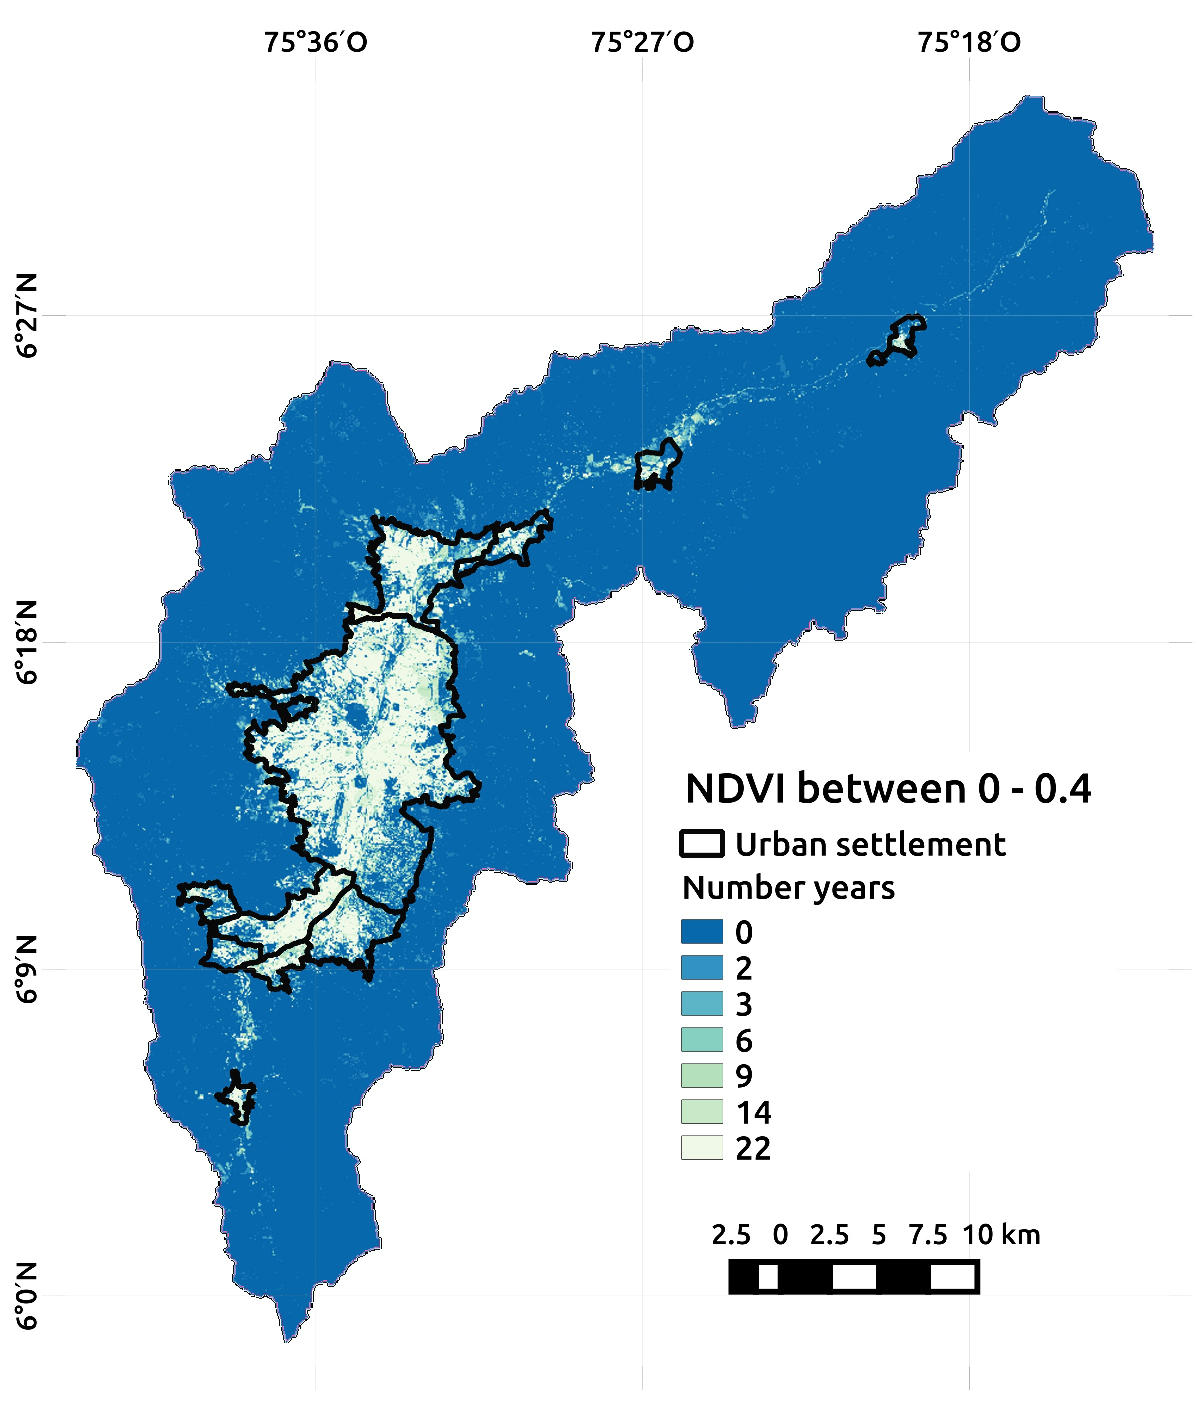
\includegraphics[trim={0.2cm 0cm 0.2cm 0cm},clip,width=8.0cm]{Figuras/evol_ndvi.pdf}
\caption{Interaccion antropica.}
\label{fig:evol_ndvi}
\end{figure}

Adicionalmente se analiza la evolución año por año de las celdas clasificadas en el rango de NDVI establecido para cada zona critica identificada en (\ref{fig:incendios_mapas}). En la figura (\ref{fig:porc_ndvi}) se presenta el crecimiento porcentual de las celdas clasificadas como desarrollo urbano en los mapas de NDVI evaluados.

\begin{figure}[h]
\centering
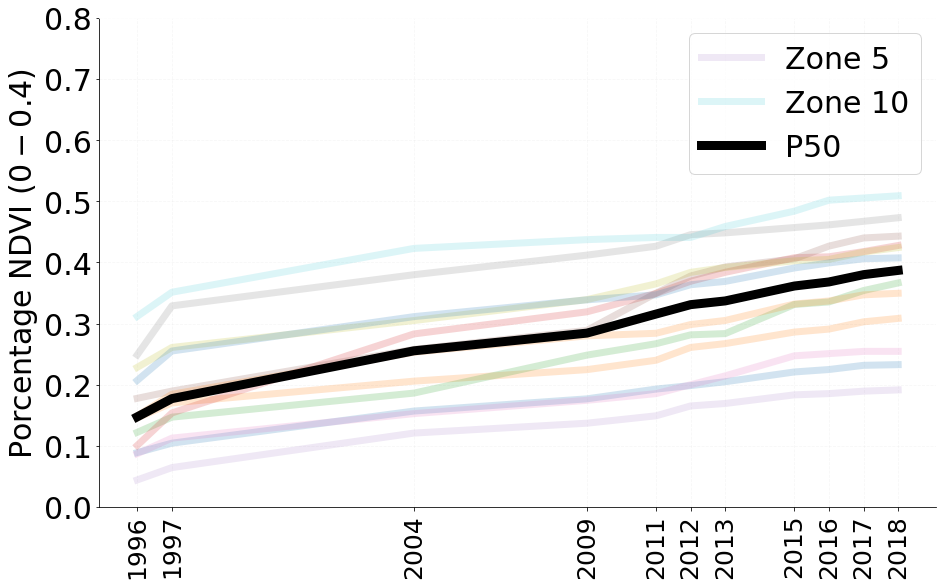
\includegraphics[trim={0.2cm 0cm 0.2cm 0cm},clip,width=9.0cm]{Figuras/porc_ndvi.png}
\caption{Interaccion antropica.}
\label{fig:porc_ndvi}
\end{figure}

El crecimiento promedio para las coberturas de suelo tipicas de desarrollo urbano o de interaccion antropica en dichas zonas es de $2\%$ cada año. Para las zonas criticas analizadas, el porcentaje de area clasificada como desarrollo urbano en el primer año esta entre $10\%$ y $50\%$.

\subsection*{Cobertura de suelo}

Para desarrollar el modelo de susceptibilidad a incendios forestales se debe considerar el tipo de cobertura en el suelo ya que condiciona la ignición del fuego y su posterior propagación, influye además en el tipo de incendio que se pueda presentar, posibilidades de extinción, formas de recuperación y valoración económica de las perdidas una vez ocurrido el evento.\\

La determinación de las coberturas es realizada por clasificación supervisada a partir de una imagen del Valle de Aburrá adquirida del satélite Pleiades de junio de 2016, con resolución espacial de $50cm$, obteniendo 6 clases de coberturas, bosques, pastos, suelo seco o desnudo, cultivo, impermeable y cuerpos de agua. Los registros historicos de incendios son relacionados con el tipo de cobertura para relacionar la probabilidad de ocurrencia de un incendio con la condicion del suelo. En la figura (\ref{fig:covert_class}) se observa que segun la historia de registros cerca del $80\%$ de los eventos ocurren en pastos, seguido de bosque con $30\%$ y en menor proporcion los cultivos y suelos desnudos.\\

Al relacionar la cobertura del suelo y la distancia al asentamiento urbano se establece que los incendios en cobertura bosque y cultivo se presentan a una mayor distancia que los ocurridos en pastos y suelo seco. La expansión urbana implica cambios en la cobertura, estas zonas de transición cercanas al asentamiento urbano estan dominadas por coberturas tipo pasto y suelo seco. Por su parte las zpnas de desarrllo agricola y las coberturas menos intervenidas (bosque) se encuentran ubicadas mas alejadas de la interaccion antropica.  


\subsection*{Ocurencia en zonas criticas}

Para completar el conjunto de variables estaticas se considera un mapa de ocurrencia histórica en el cual las zonas criticas del Valle de Aburra toman mayor importacia. Este mapa agrega susceptibilidad adicional a aquellas zonas donde históricamente se presentan mayor cantidad de incendios y la disminuye para las zonas donde es muy poco frecuente la ocurrencia de este tipo de eventos.


En la seccion de metodologia se incluyen las variables estaticas descritas en esta sección; interaccion antropica, cobertura de suelo y ocurrencia en zonas criticas como aporte a la estimacion de susceptibilidad a incendios forestales.

\begin{figure}[h]
\centering
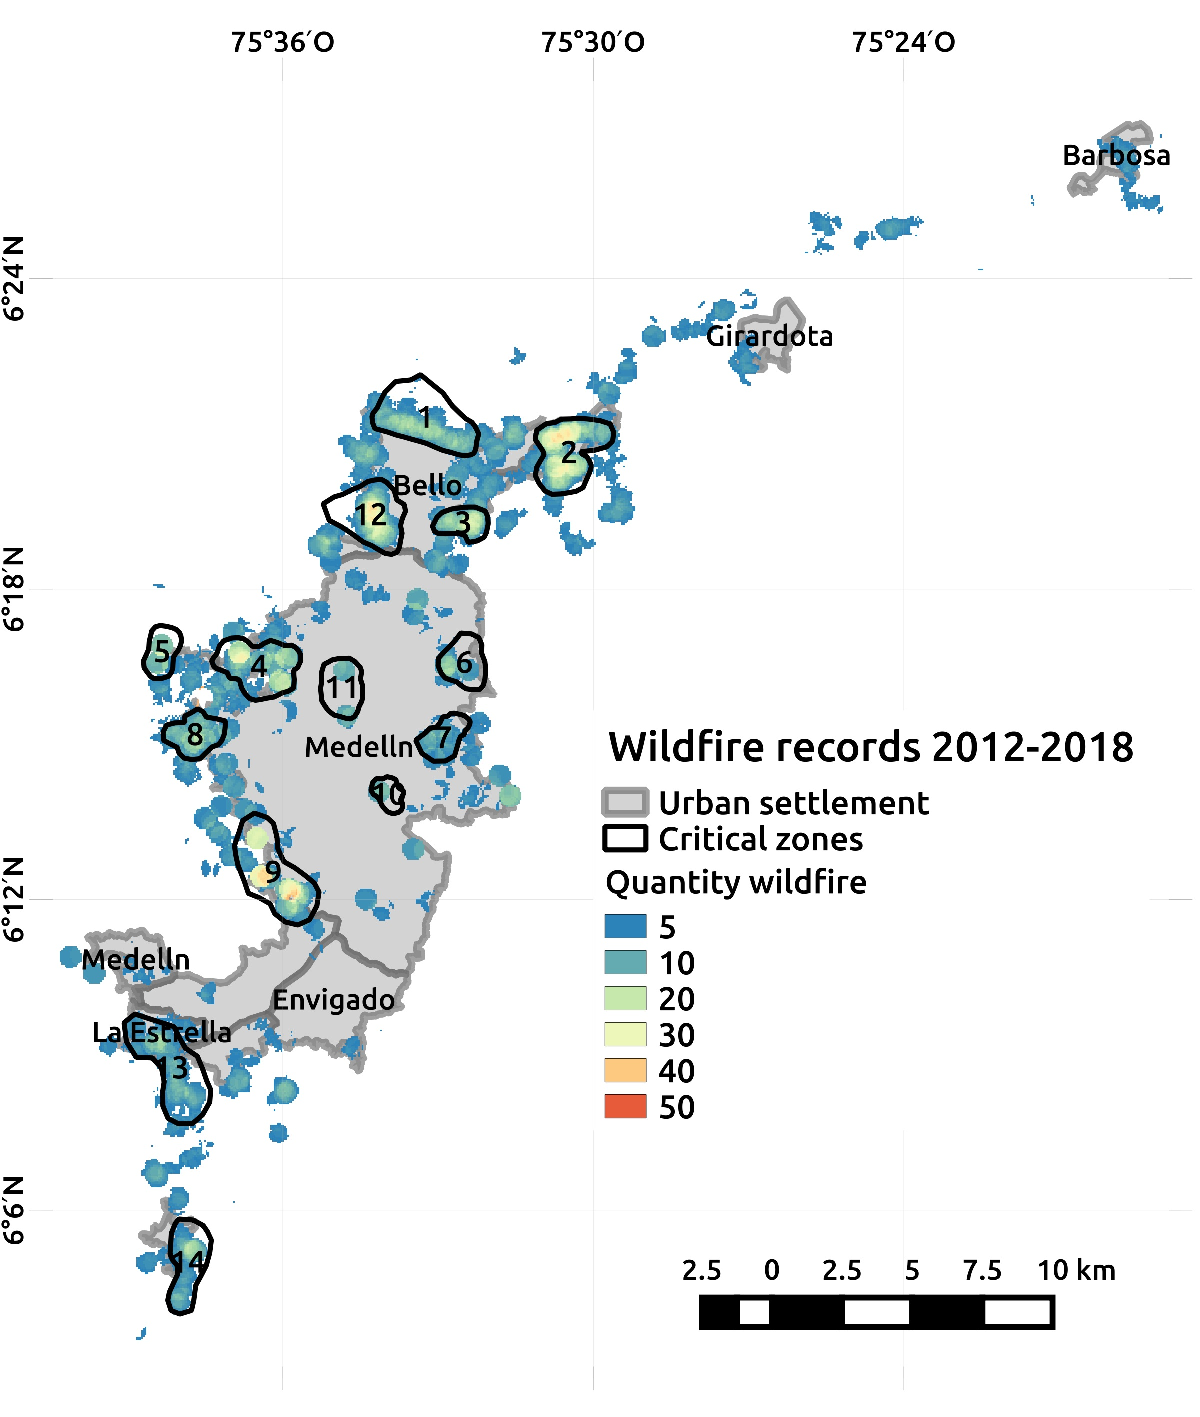
\includegraphics[width=8.cm]{Figuras/map_intro.pdf}
\caption{Evolution of the number of forest fire events reported at the VA in the last N years.}
\label{fig:incendios_mapas}
\end{figure}

\subsection{Dynamic Data}

\subsection*{Precipitación}

Desde el punto de vista climático la precipitación es una de las variables mas determinantes para estimar la vulnerabilidad y disposición de los materiales a ser encendidos. Para el Valle de Aburrá se dispone de registros de precipitación obtenidos del radar meteorológico operado por el SIATA con resolución temporal de cinco minutos y espacial de aproximadamente 150 metros. Para el planteamiento del modelo de susceptibilidad se considera la precipitación desde dos puntos de vista:

Acumulado de precipitación: se calculan acumulados de precipitación para una ventana de tiempo previa a la ocurrencia de los incendios reportados en la base historica con el objetivo de encontrar un patrón relacionado con la precipitación precedente. La ventana de tiempo para calcular le precipitación acumulado fue variada desde 5 hasta 30 días para buscar la relación mas clara. Las precipitaciones acumuladas presentan una distribución particular para los días con ocurrencia de incendio. Se establece que 10 días es una ventana de tiempo adecuada para diferenciar los acumulados entre días de ocurrencia de incendio y los demás registros. El 70\% de los incendios ocurrieron para acumulados menores a  $60mm$  en los últimos 10 días (Figura \ref{fig:dynamic_rain}).

Días de sequía antecedente: se calculan los días de sequía precedentes al día del incendio. En el item anterior se establece que para el  $70\%$ de los incendios el acumulado de precipitación no supera los  $60mm$  en 10 días, esta valor es empleado como umbral para establecer los días antecedentes al incendio que fueron necesarios para superarlo.

\begin{figure*}
\centering
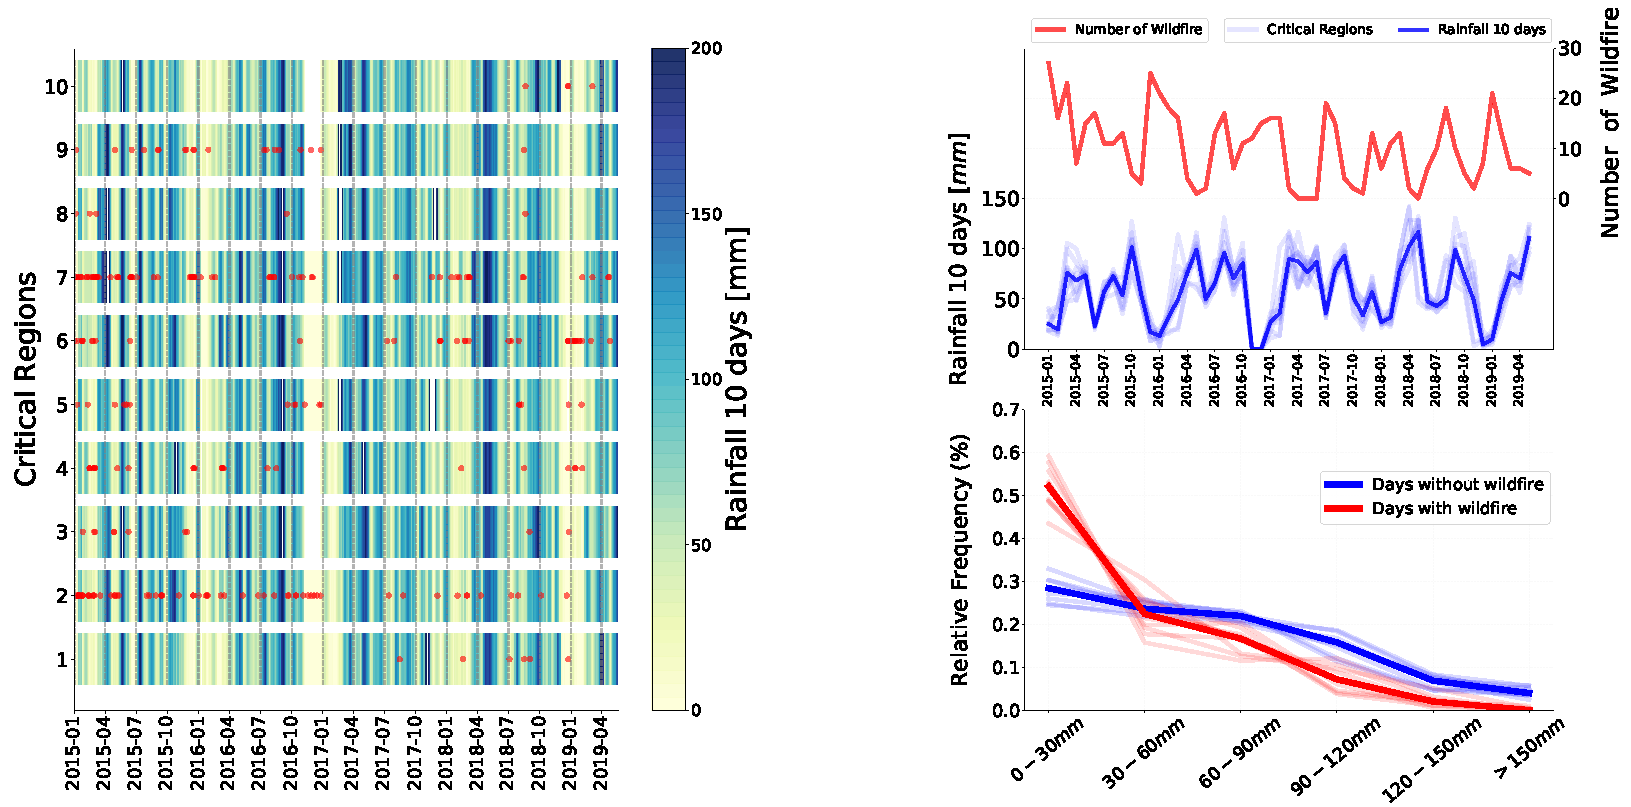
\includegraphics[width=18.cm]{Figuras/rain_composition.pdf}
\caption{Evolution of the number of forest fire events reported at the VA in the last N years.}
\label{fig:dynamic_rain1}
\end{figure*}

\subsection*{Humedad del suelo}

La humedad del suelo es una variable determinante en la ignición de incendios y esta ligada a las condiciones de precipitación. La humedad del suelo se hace importante debido a que representa las condiciones en superficie de los materiales de cobertura (combustible) en función de las características topográficas y geomorfológicas de la zona (Figura \ref{fig:dynamic_moisture}). 

En el modelo se susceptibilidad de incendios se incorpora esta variable para representar las características físicas del terreno en cuanto al almacenamiento capilar el cual presenta un comportamiento variable en el espacio.

Para determinar la humedad en el suelo se emplean los resultados del modelo hidrológico distribuido que es operado en el SIATA. En este modelo se simulan de manera distribuida los procesos hidrológicos mas importantes siendo uno de ellos el almacenamiento capilar. 

Para establecer las condiciones de humedad del suelo relacionas a la ocurrencia de un incendio se evalúa la distribución de dicha variable para los incendios históricos.

\subsection*{Temperatura}

Para el historico de incendios se estima la temperatura superficial del punto en que ocurrieron en base a la temperatura ambiente monitoreada en SIATA. Estas estimaciones se emplean para determinar un valor mínimo de temperatura necesario para la ocurrencia de incendios, el cual se utiliza como filtro en el modelo operacional de incendios forestales (Figura \ref{fig:dynamic_temp}).


\section{RESULTADOS}

\begin{figure}[h]
\centering
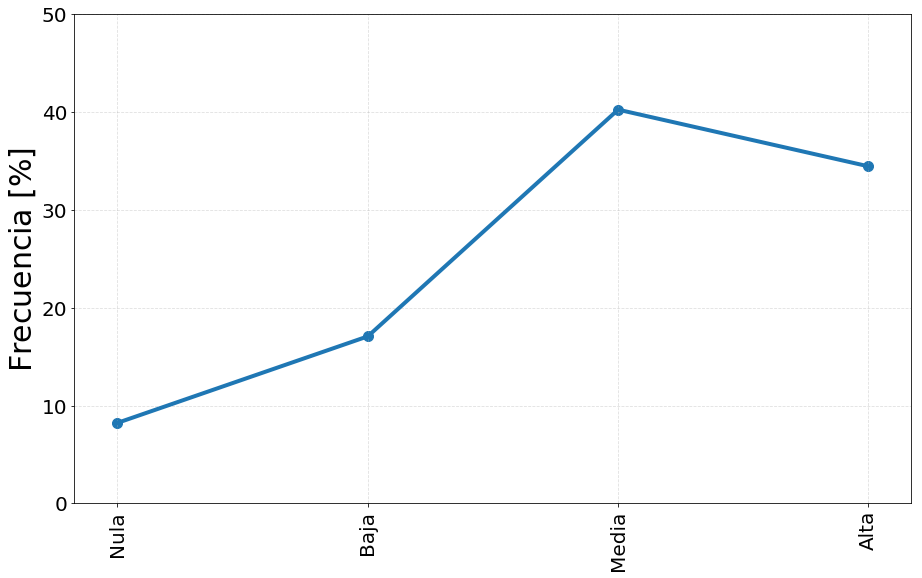
\includegraphics[trim={0.2cm 0cm 0.2cm 0cm},clip,width=8.6cm]{Figuras/susc_events.png}
\caption{Susceptibilidad a incendios forestales estimada por el modelo para 328 eventos ocurridos entre 2018-01-01 y 2019-02-01.}
\label{fig:temp_IPCC}
\end{figure}

\begin{figure}[h]
\centering
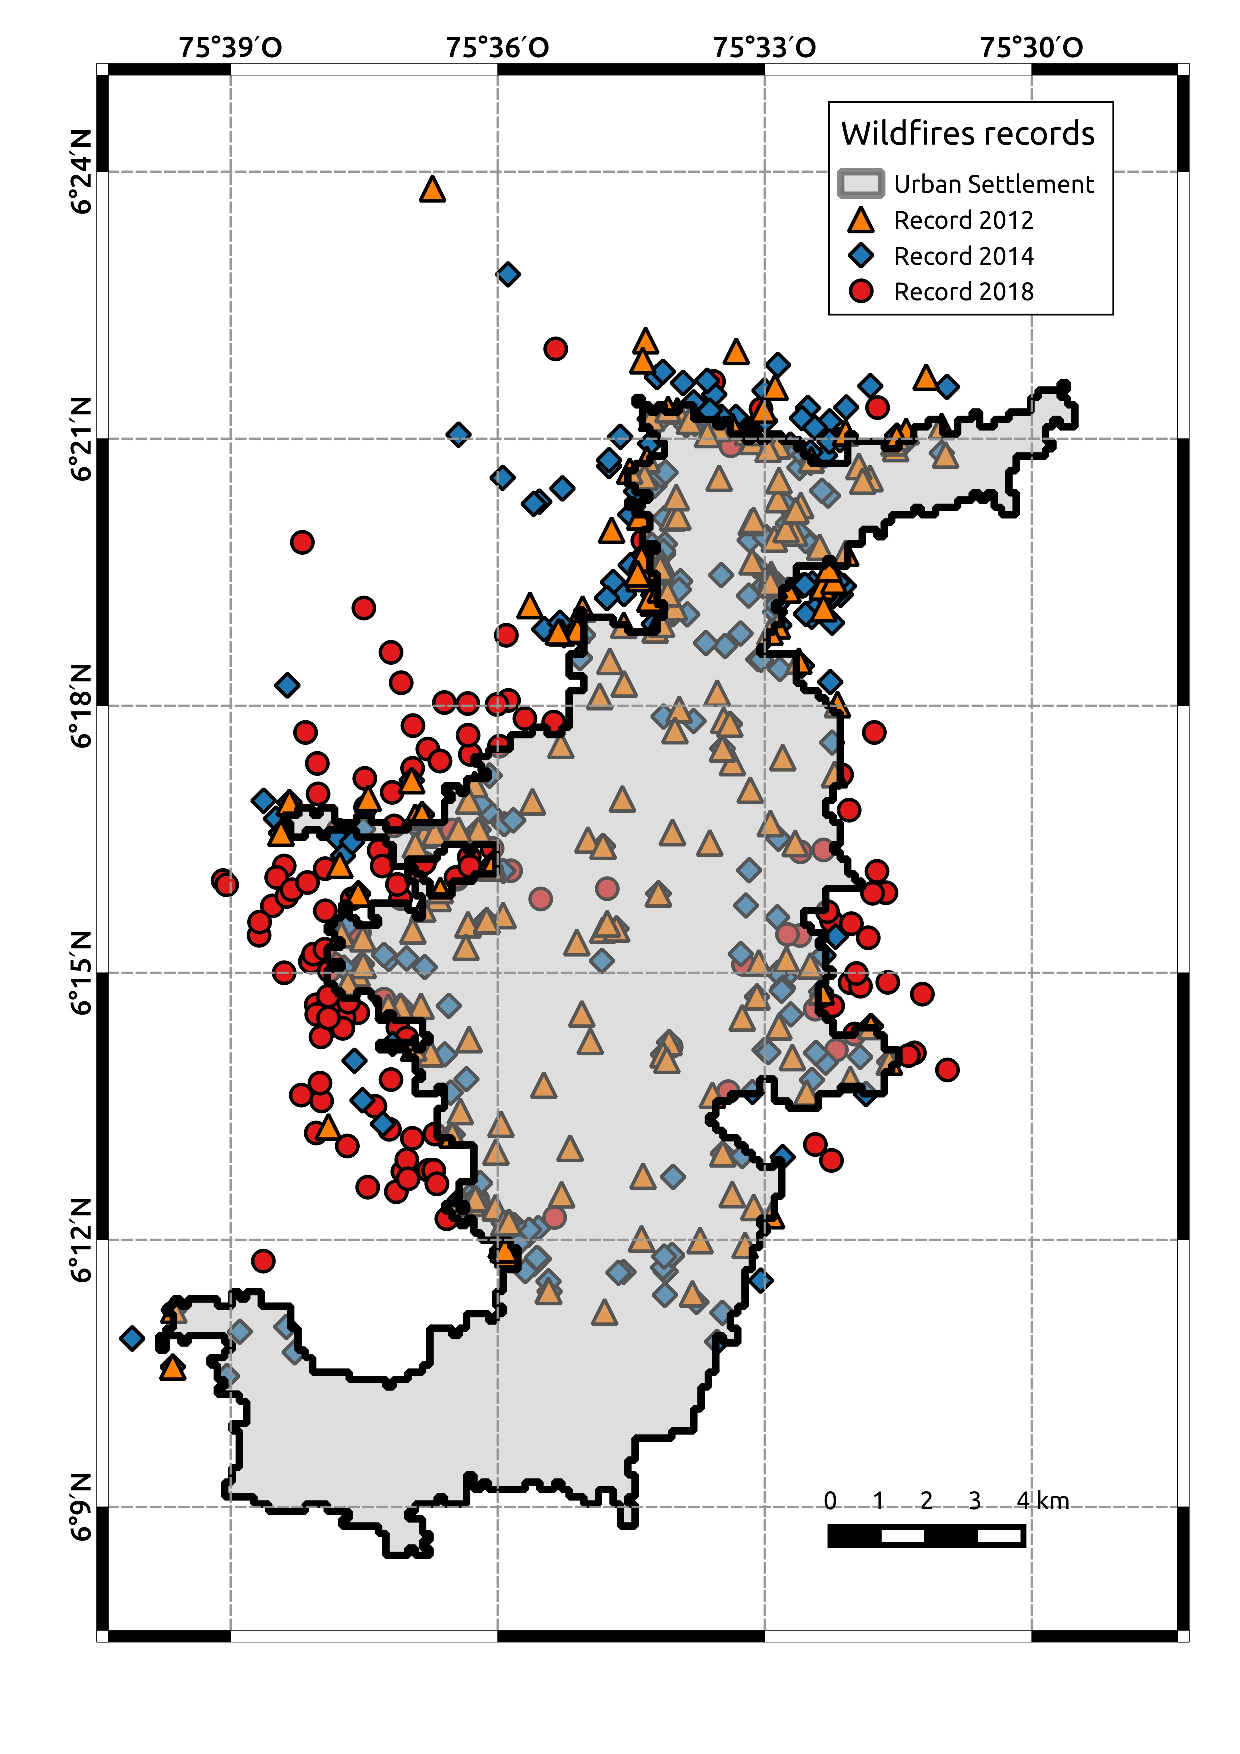
\includegraphics[trim={0.2cm 0cm 0.2cm 0cm},clip,width=8.6cm]{Figuras/map_wildfires.pdf}
\caption{Susceptibilidad a incendios forestales estimada por el modelo para 328 eventos ocurridos entre 2018-01-01 y 2019-02-01.}
\label{fig:map_wildfire}
\end{figure}

%\input{conclusiones.tex}

\addcontentsline{toc}{chapter}{\numberline{}Bibliografía}

\bibliographystyle{apalike}
\bibliography{BibliMSc}



\end{document}
